\documentclass[11pt]{article}
\usepackage[margin=1in]{geometry}
\usepackage{amsmath,amssymb,amsthm,mathtools}
\usepackage{graphicx}
\usepackage{hyperref}
\usepackage{xcolor}

\newtheorem{theorem}{Theorem}
\newtheorem{proposition}[theorem]{Proposition}
\newcommand{\C}{\mathbb C}

\title{A Multiplicity Counterexample to a Uniform\\
Many-Polynomial B\'ezout Estimate}
\author{Automatic mathematics run \texttt{fa\_banach\_001}}
\date{9 August 2026}

\begin{document}
\setlength{\emergencystretch}{3em}
\maketitle

\begin{center}
\fbox{\parbox{0.91\textwidth}{
\textbf{Status.} Candidate counterexample, likely valid, for human review.
It gives a full negative answer to the open problem in Section 10.4 of
Fricain--Hartmann--Ross--Timotin as the problem is stated.
}}
\end{center}

\section{Source problem}

Fricain, Hartmann, Ross, and Timotin study coefficient-norm estimates for
polynomial B\'ezout identities \cite{source}.  For
\(A_1,\ldots,A_q\in\C[z]\) with no common zero, they define
\[
 \delta=\min\left\{
       \sum_{i=1}^q |A_i(z)|:
       z\in\C,\ \prod_{i=1}^q A_i(z)=0
     \right\}.
\]
Their Section 10.4 asks for a constant \(C>0\), depending only on
\(\max_i\deg A_i\), such that one can solve
\[
 \sum_{i=1}^q A_iR_i=1
 \qquad\text{with}\qquad
 \max_i\|R_i\|\le \frac{C}{\delta^2},                 \tag{1}
\]
where \(\|R\|\) is the maximum modulus of the coefficients of \(R\).
The preceding paragraph also gives the usual degree restriction
\(\deg R_i\le\max_j\deg A_j-1\).

The complete source page follows.  Notice especially that \(C\) may depend
on the maximal degree but not on the number \(q\) of polynomials.

\clearpage
\begin{center}
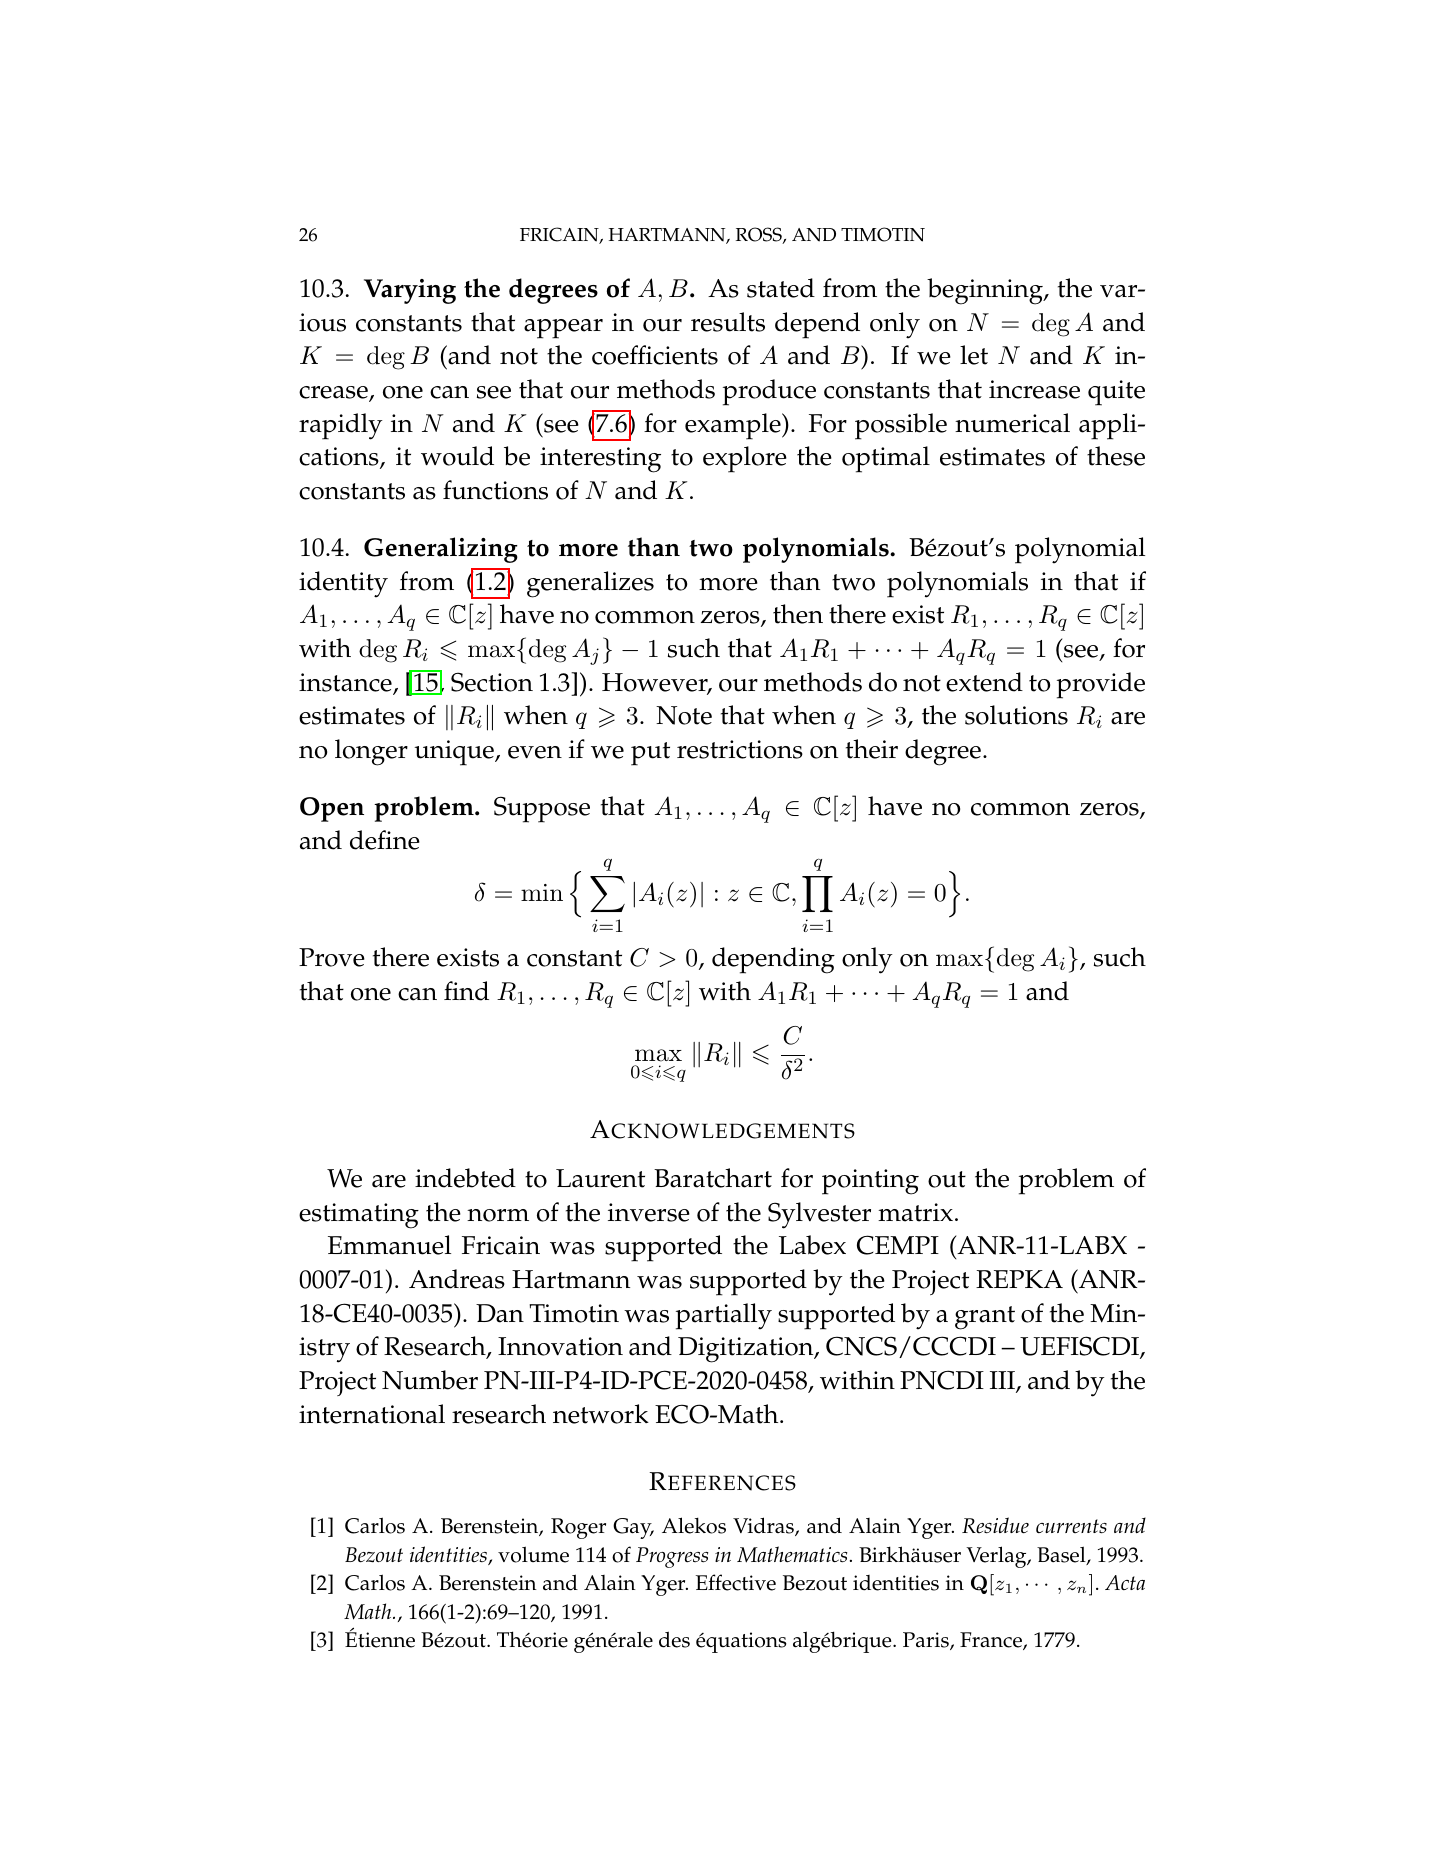
\includegraphics[width=0.96\textwidth]{figures/source_open_problem_page26.png}
\end{center}

\section{Counterexample}

The obstruction is duplication.  The definition of \(\delta\) adds the
moduli of all inputs, so repeating generators makes \(\delta\) grow linearly.
But repeating a generator can reduce the largest B\'ezout coefficient only
linearly, whereas (1) demands a quadratic reduction.

\begin{theorem}\label{thm:counterexample}
There is no constant in \emph{(1)} depending only on the maximal degree.
This remains false under the normalization \(\|A_i\|\le1\), and remains false
even if the solution polynomials \(R_i\) are allowed arbitrary degrees.
\end{theorem}

\begin{proof}
Let \(m\ge1\), put \(q=2m\), and define
\[
 A_1=\cdots=A_m=z,
 \qquad
 A_{m+1}=\cdots=A_{2m}=1-z.                              \tag{2}
\]
These polynomials have no common zero, their maximal degree is one, and every
one of them has coefficient norm exactly one.

The product in the definition of \(\delta\) vanishes precisely at \(z=0\)
and \(z=1\).  At either point exactly \(m\) summands in
\(\sum_i|A_i(z)|\) equal one and the other \(m\) vanish.  Consequently
\[
 \delta=m.                                                \tag{3}
\]

Consider any polynomial solution \(R_1,\ldots,R_{2m}\) of the B\'ezout
identity for (2).  Evaluating it at \(z=0\) gives
\[
 \sum_{i=m+1}^{2m}R_i(0)=1.                              \tag{4}
\]
It follows from the triangle inequality that
\[
 1\le \sum_{i=m+1}^{2m}|R_i(0)|
   \le m\max_{m<i\le2m}\|R_i\|,
\]
and hence
\[
 \max_{1\le i\le2m}\|R_i\|\ge \frac1m.                \tag{5}
\]
This argument uses only constant terms, so allowing higher degrees does not
help.  (Evaluation at \(z=1\) gives the same lower bound on the first block.)

If (1) held, maximal degree one would determine a single constant \(C\),
independent of \(m\).  Equations (3) and (5) would give
\[
 \frac1m\le \max_i\|R_i\|\le\frac{C}{m^2}.
\]
Choosing an integer \(m>C\) is a contradiction.
\end{proof}

\section{Exact obstruction and necessary repair}

The preceding lower bound is not an artifact of the proof.

\begin{proposition}
For the family \emph{(2)}, the minimum possible value of
\(\max_i\|R_i\|\), over all polynomial B\'ezout solutions, is exactly
\[
 \frac1m=\frac{q}{2\delta^2}.                            \tag{6}
\]
\end{proposition}

\begin{proof}
The lower bound is (5).  For equality, take the constant polynomial
\(R_i=1/m\) for every \(i\).  Then
\[
 \sum_{i=1}^{2m}A_iR_i
 =m z\frac1m+m(1-z)\frac1m=1.
\]
Since \(q=2m\) and \(\delta=m\), this optimum equals the right-hand side
of (6).
\end{proof}

Thus a repaired estimate of the form
\(C(q,d)\delta^{-2}\) must have \(C(q,1)\ge q/2\) along even values of
\(q\).  Equivalently, if the \(\ell^1\)-type separation parameter in the
source is retained, at least linear dependence on the number of generators
is unavoidable.  The example does not decide whether a bound with linear
\(q\)-dependence is sufficient in general, nor does it address the sharp
dependence on \(\delta\) when \(q\) is fixed.

\section{Verification and novelty scope}

The proof reduces to the exact identities (3)--(5).  An independent script
checks the source parameter, the explicit extremal solution, and (6) with
exact rational arithmetic for \(1\le m\le10{,}000\).  The computation is a
sanity check and is not used in the proof.

A bounded literature audit was performed on 9 August 2026 after the direct
argument: the run indexes, exact-phrase and core-keyword web searches, the
current arXiv record, and author/citation search pages were checked.  No later
answer or occurrence of this duplication example was found.  Novelty is
therefore plausible, not certified.

\begin{thebibliography}{9}
\bibitem{source}
E. Fricain, A. Hartmann, W. T. Ross, and D. Timotin,
\emph{An analytic approach to estimating the solutions of B\'ezout's
polynomial identity}, arXiv:2310.12734v3 (2024).
\end{thebibliography}

\end{document}
